\subsection{Evaluated Experimental Layout}

This is a preserved simulation layout, not a recommendation to install barriers. The practical review below rejects those belts as an installation proposal. The selected experimental candidate uses the same six posts as the reference. CM2, CM3, CM5 and CM6 recommend the foyer; the end posts retain portico messages. All four factorial policies use these coordinated messages. The original-message baseline is an additional control. Locations below are graph junctions, not surveyed installation coordinates.

\begin{table}[htbp]\centering\small

\begin{tabular}{lll}\toprule

Manager & Junction & Public recommendation\\\midrule

CM1 & \texttt{m1} & west portico\\

CM2 & \texttt{m4} & foyer\\

CM3 & \texttt{m8} & foyer\\

CM4 & \texttt{m11} & east portico\\

CM5 & \texttt{b4} & foyer\\

CM6 & \texttt{b8} & foyer\\

\bottomrule\end{tabular}\caption{Fixed six-manager arrangement for the intervention arms.}\end{table}

\begin{table}[htbp]\centering\small

\begin{tabular}{rlll}\toprule

LED & Junction & Installed walkway & Initial public message\\\midrule

1 & \texttt{m1} & \texttt{mezzanine-1} & west portico\\

2 & \texttt{m3} & \texttt{mezzanine-3} & foyer\\

3 & \texttt{m5} & \texttt{mezzanine-5} & foyer\\

4 & \texttt{m7} & \texttt{mezzanine-7} & foyer\\

5 & \texttt{m9} & \texttt{mezzanine-9} & foyer\\

6 & \texttt{m11} & \texttt{mezzanine-11} & east portico\\

7 & \texttt{b1} & \texttt{balcony-1} & northwest balcony\\

8 & \texttt{b4} & \texttt{balcony-4} & foyer\\

9 & \texttt{b7} & \texttt{balcony-7} & foyer\\

10 & \texttt{b10} & \texttt{balcony-10} & northeast balcony\\

11 & \texttt{c1} & \texttt{corridor-1} & west portico\\

12 & \texttt{c4} & \texttt{corridor-4} & foyer\\

13 & \texttt{c7} & \texttt{corridor-7} & foyer\\

14 & \texttt{c10} & \texttt{corridor-10} & east portico\\

15 & \texttt{oL0} & \texttt{inner-L-1} & west stage\\

16 & \texttt{oR0} & \texttt{inner-R-1} & east stage\\

\bottomrule\end{tabular}\caption{Sixteen dynamic strip installations. The controller may change messages through the delayed observation and holding rules; messages are not personalized.}\end{table}

The two side-anchored open belts occupy \texttt{corridor-3} and \texttt{corridor-8}. Each is 1 m long at $30^\circ$ to its corridor direction. Its projected span is 0.5 m, leaving 1.9 m of the assumed 2.4 m width; the lane count falls from four to three. Both travel directions remain allowed. The altered polyline includes a free-end bypass detour. These are low/open devices with no opaque panel or added sightline obstacle. Wheelchair and all-origin connectivity are checked. Neither belt occupies a door threshold.

\begin{figure}[htbp]\centering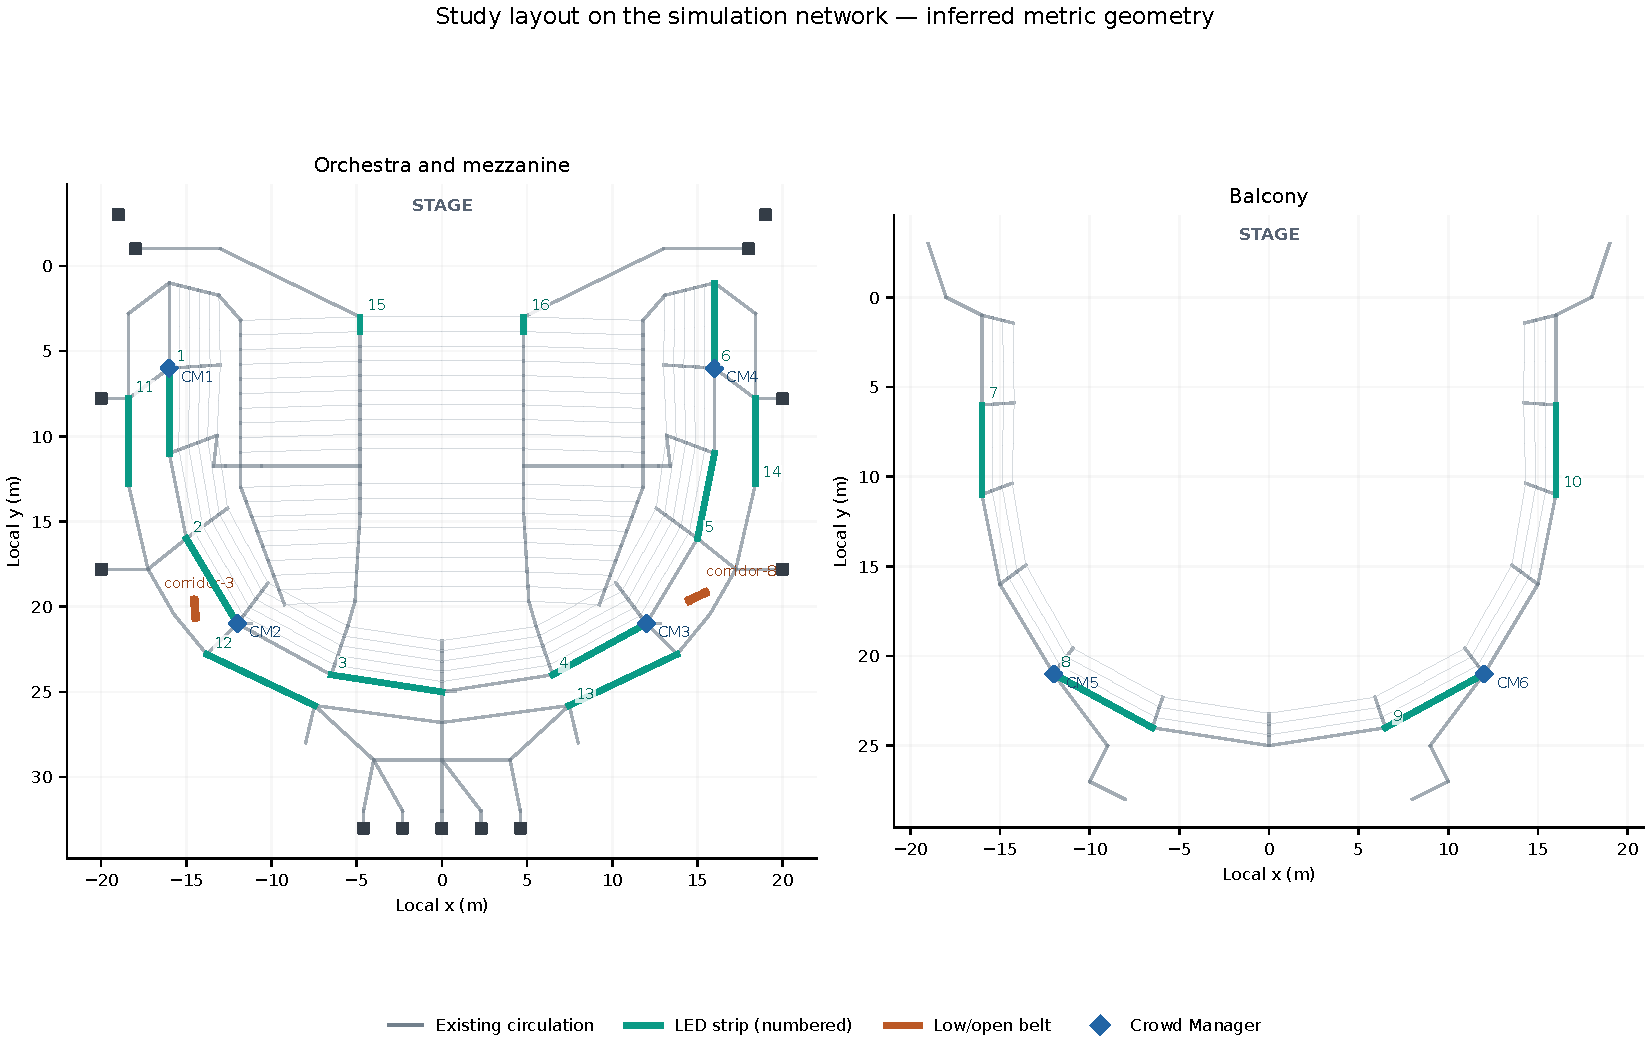
\includegraphics[width=\linewidth]{figures/intervention-layout.pdf}

\caption{Installation schematic generated from the same network as the simulation. Numbers identify the LED strips in the table. Belts preserve views but still consume physical width. Metric reconstruction and installation feasibility require venue verification.}\end{figure}
